\section{Search}
BFS, DFS, UCS, A*. For A* to work, the heuristic gotta be admissible (heuristic is always less than or equal to true cost to the end) and consistent (cost from $a$ to $b$ is $c$, $h(a) - h(b) \leq c$).

Examples:

\begin{figure}[H]
    \centering
    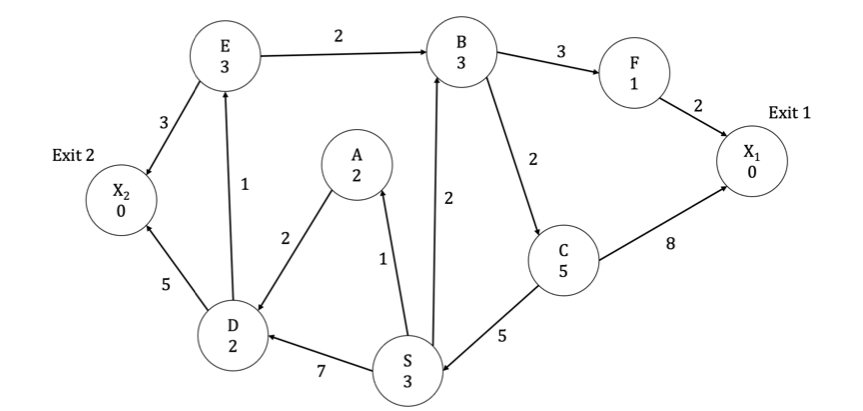
\includegraphics[width=\linewidth]{graph}
\end{figure}

\textbf{BFS:} exit node $X_2$, path $S, A, B, D$

\textbf{DFS:} exit node $X_2$, path $S, A, D$

\textbf{UCS:} exit node $X_1$, path $S, A, B, D, C, E, F, X_1$

\textbf{A*:} exit node $X_1$, path $S, A, B, D, F, E, X_1$
